\chapter{Implementacija i korisničko sučelje}
		
		
		\section{Korištene tehnologije i alati}
			 
			 Komunikacija u timu realizirana je korištenjem aplikacija \underbar{WhatsApp}\footnote{\url{https://www.whatsapp.com/}} i \underbar{Discord}\footnote{\url{https://discord.com/}}. Za izradu dijagrama korištena je aplikacija \underbar{Astah Proffesional}\footnote{\url{https://astah.net/products/astah-professional/}}, a za pisanje dokumenatcije korišten je opisni jezik \underbar{LaTeX}\footnote{\url{https://www.latex-project.org/}} u aplikaciji \underbar{TeXstudio}\footnote{\url{https://www.texstudio.org/}}. kao sustav za upravljanje izvornim kodom koristo se sustav \underbar{Git}\footnote{\url{https://git-scm.com/}}. Udaljeni repozitorij projekta je dostupan na web platformi \underbar{GitHub}\footnote{\url{https://github.com/}}.
			 
			 Kao razvojno okruženje koristili smo \underbar{Visual Studio Code}\footnote{\url{https://code.visualstudio.com/}}. Visual Studio Code je uređivač koda kojeg je razvio Microsoft za Windows, Linux i MacOs operacijske sustave. Olakšava rad s Gitom i omogućava pokretanje programa. Omogućava i instaliranje exstenzija za lakši rad s različitim programskim jezicima i radnim okvirima.
			 
			 Aplikacija je pisana koristeći radni okvir \underbar{Flask}\footnote{\url{https://flask.palletsprojects.com/}}, \underbar{SQLAlchemy}\footnote{\url{https://www.sqlalchemy.org/}} i jezik \underbar{Python}\footnote{\url{https://www.python.org/}} za izradu \textit{backenda}, te \underbar{React}\footnote{\url{https://react.dev/}} i jezik \underbar{JavaScript}\footnote{\url{https://www.javascript.com/}}. Flask je mikro radni okvir koji pruža osnovne funkcionalnosti za razvoj web-aplikacija, ali i omogućava programeru određenu razinu slobode. React, poznatiji kao ReactJS ili React.js je biblioteka u javascriptu koja omogućava izgradnju korisničkih sučelja, održavana od strane Facebooka.
			 
			 Baza podataka nalazi se na \underbar{Renderu}\footnote{\url{https://render.com/}}.
			
			
			\eject 
		
	
		\section{Ispitivanje programskog rješenja}
			
			\subsection{Ispitivanje komponenti}
			
			U ovom odjeljku je opisano izvršavanje testova za testiranje ispravnosti sučelja poslužitelja. 
			
			
			\textbf{Incijalizacija}
			
			
			Kako bi postavili testno okruženje i pokrenuli tesnog poslužitelja vršimo kod:
			
			\begin{figure}[H]
				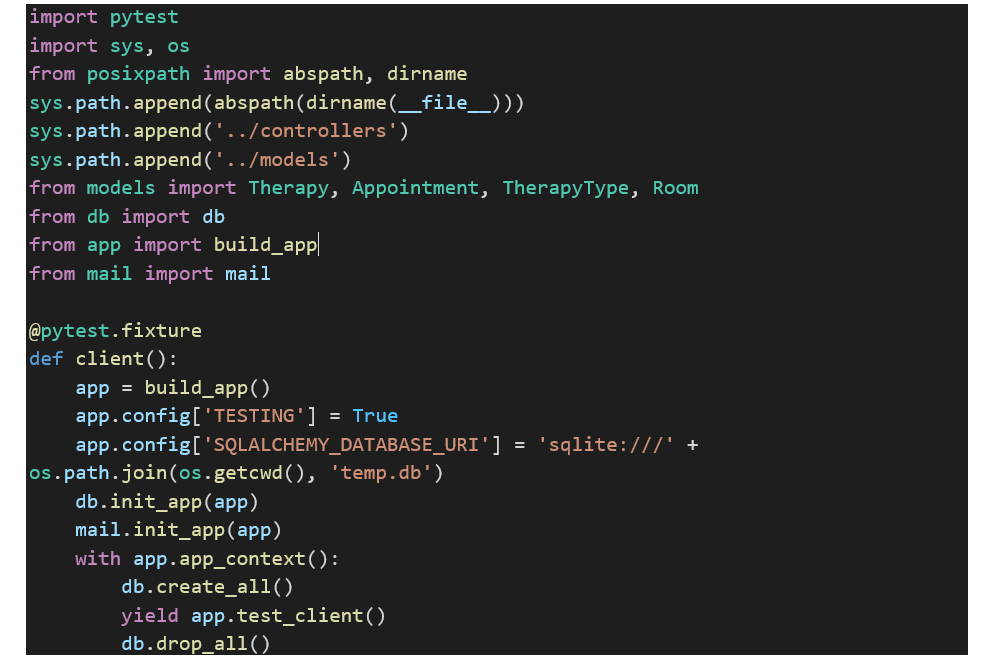
\includegraphics[scale=0.3]{slike/testno_okruzenje.PNG} %veličina slike u odnosu na originalnu datoteku i pozicija slike
				\centering
				\caption{Inicijalizacija testnog okruženja}
				\label{fig:testno_okruzenje}
			\end{figure}
			
			U prvom dijelu se definiraju korišteni moduli, a drugom dijelu se definira funkcija \textit{client} koja vraća instancu poslužitelja koju je onda moguće koristiti za testiranje. U funkciji se stvara prazna privremena baza podataka na istoj memorijskoj lokaciji. \\
S naredbama \texttt{db.init\_app(app)} će se inicijalizirati baza podataka po uzoru na db objekt koji sadrži sve entitete u poslužitelju. \texttt{mail.init\_app(app)} služi kako bi se omogućilo slanje obavijesti na e-poštu. Iako se ono ne provjerava tijekom testiranja, potrebno je za ispravan rad aplikacije. \\
Ova funkcija će se pokrenuti prije svakog testa kako bi se baza podataka očistila i time testovi ne bi utjecali jedni na druge.


\textbf{Testovi}


U testovima će se uglavnom testirati manipulacija terminima jer je to najsloženija procedura.

            \begin{figure}[H]
				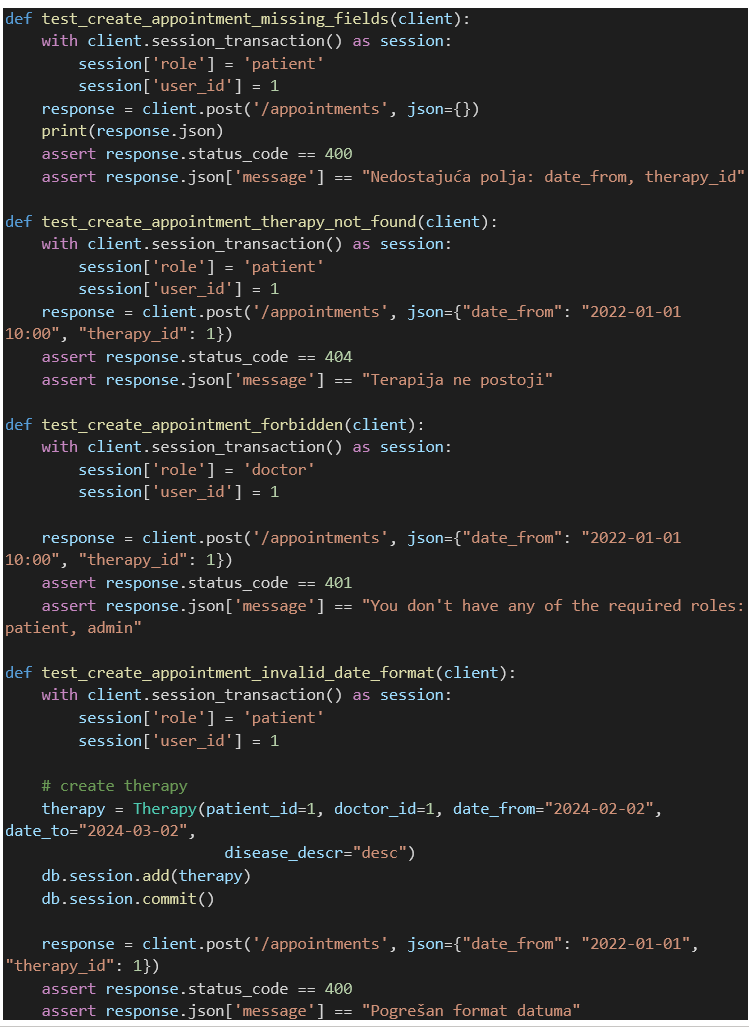
\includegraphics[scale=0.3]{slike/testovi_1_2_3_4.PNG} %veličina slike u odnosu na originalnu datoteku i pozicija slike
				\centering
				\caption{Testovi 1, 2, 3 i 4}
				\label{fig:testovi1234}
			\end{figure}
			
			\begin{figure}[H]
				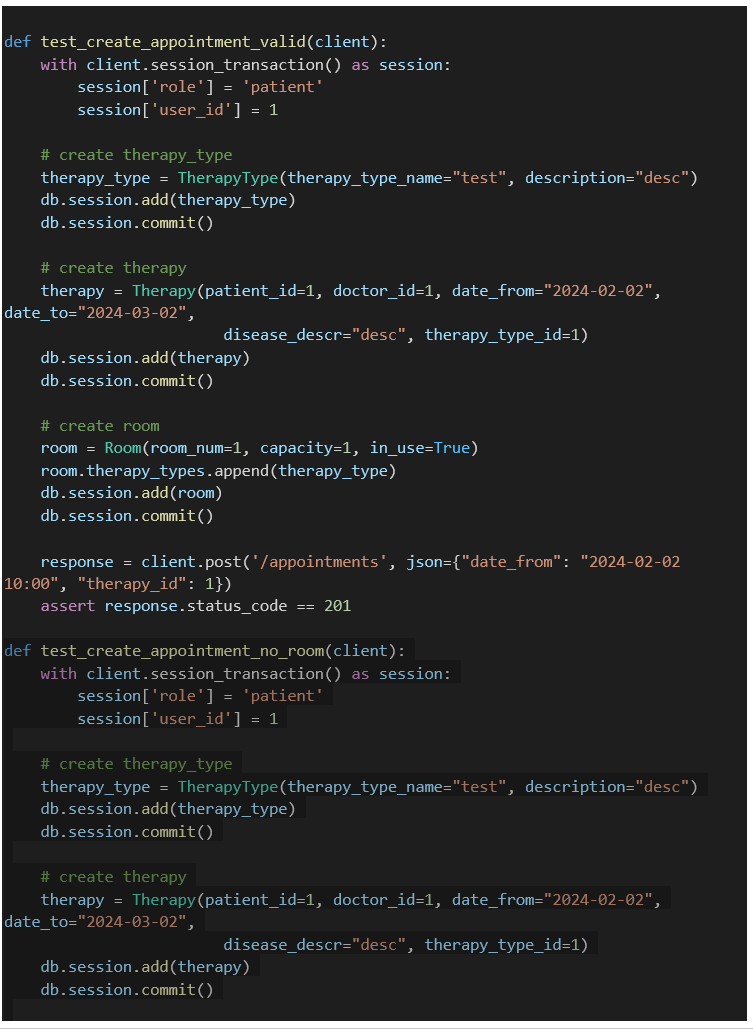
\includegraphics[scale=0.3]{slike/testovi_5_6dio.PNG} %veličina slike u odnosu na originalnu datoteku i pozicija slike
				\centering
				\caption{Testovi 5 i 6a}
				\label{fig:testovi56a}
			\end{figure}
			
			\begin{figure}[H]
				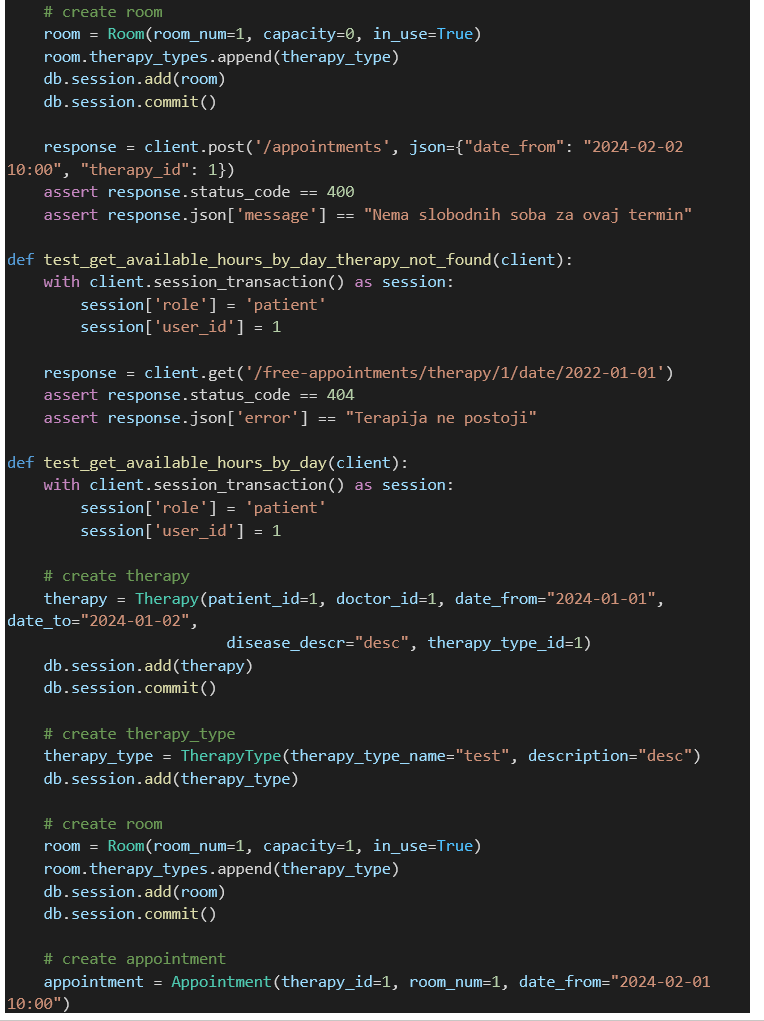
\includegraphics[scale=0.3]{slike/testovi_6dio_7_8dio.PNG} %veličina slike u odnosu na originalnu datoteku i pozicija slike
				\centering
				\caption{Testovi 6b, 7 i 8a}
				\label{fig:testovi6b78a}
			\end{figure}
			
			\begin{figure}[H]
				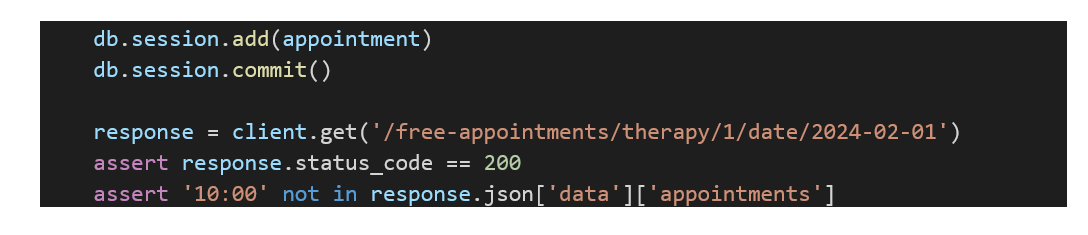
\includegraphics[scale=0.3]{slike/testovi_8dio.PNG} %veličina slike u odnosu na originalnu datoteku i pozicija slike
				\centering
				\caption{Test 8b}
				\label{fig:testovi8b}
			\end{figure}
			
			
	\begin{packed_item}
		\item \texttt{test\_create\_appointment\_missing\_fields(client)} \\
Testira hoće li funkcija za stvaranje termina (putem HTTP POST zahtjeva) vratiti status 400 i odgovarajuću poruku ako nedostaju polja \texttt{date\_from} i \texttt{therapy\_id}.
		\item \texttt{test\_create\_appointment\_therapy\_not\_found(client)} \\
		Provjerava hoće li funkcija vratiti status 404 i odgovarajuću poruku ako terapija s navedenim ID-jem ne postoji.
        \item \texttt{test\_create\_appointment\_forbidden(client)} \\
        Testira hoće li funkcija vratiti status 401 i odgovarajuću poruku ako korisnik koji pokušava stvoriti termin nema ulogu pacijenta ili administratora.
        \item \texttt{test\_create\_appointment\_invalid\_date\_format(client)} \\
        Provjerava hoće li funkcija vratiti status 400 i odgovarajuću poruku ako je format datuma neispravan prilikom stvaranja termina.
        \item \texttt{test\_create\_appointment\_valid(client)} \\
        Testira uspješno stvaranje termina (status 201) kada su svi uvjeti zadovoljeni, uključujući postojanje terapije, tipa terapije, sobe i slobodnih termina.	
        \item \texttt{test\_create\_appointment\_no\_room(client)}	\\
        	Provjerava hoće li funkcija vratiti status 400 i odgovarajuću poruku ako nema slobodnih soba za navedeni termin.
        \item \texttt{test\_get\_available\_hours\_by\_day\_therapy\_not\_found(client)} \\
        Testira hoće li funkcija za dobivanje slobodnih termina po danu vratiti status 404 i odgovarajuću poruku ako terapija s navedenim ID-jem ne postoji.
        \item texttt{test\_get\_available\_hours\_by\_day(client)} \\
        Provjerava ispravno dobivanje slobodnih termina (status 200) za određeni dan, uz pretpostavku da postoji terapija, tip terapije, soba i već stvoren termin na taj dan.
                   				
	 \end{packed_item}
	 
	 \textbf{Rezultati}
	 
	 
	 Svi testovi su usješno riješeni.
	 
	 \begin{figure}[H]
				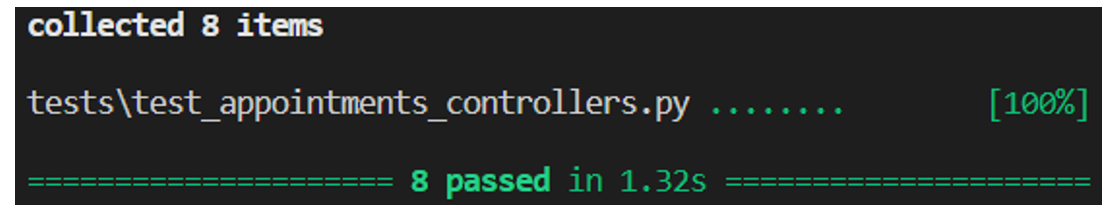
\includegraphics[scale=0.3]{slike/rezultati_testova.PNG} %veličina slike u odnosu na originalnu datoteku i pozicija slike
				\centering
				\caption{Rezultati testova}
				\label{fig:rezultati_testova}
			\end{figure}
	 
	 
			

			
			\subsection{Ispitivanje sustava}
			

\textbf{Slučaj 1: Prijava u aplikaciju kao admin, pregled svih kartica aplikacije i odjava iz aplikacije}
\textbf{Ulaz:}
\begin{enumerate}
    \item Otvaranje početne stranice u web pregledniku.
    \item Upisivanje adrese e-pošte i lozinke admina te stisak na gumb prijava.
    \item[3.a] Stisak na stranicu 'Pacijenti'
    \item[3.b] Stisak na stranicu 'Evidentiraj'
    \item[3.c] Stisak na stranicu 'Inventar'
    \item[3.d] Stisak na stranicu 'Prostorije'
    \item[3.e] Stisak na stranicu 'Korisnički račun'
    \item[4.] Stisak na opcije
    \item[5.] Stisak na gumb 'Odjavi se'
\end{enumerate}
\textbf{Očekivani rezultat:}
\begin{enumerate}
    \item Početna stranica se otvara u web pregledniku.
    \item Otvara se početna stranica aplikacije.
    \item Redom se otvaraju stranice 'Pacijenti', 'Evidentiraj', 'Inventar', 'Prostorije', 'Korisnički račun'.
    \item Otvara se padajući izbornik s opcijama.
    \item Otvara se stranica za prijavu.
\end{enumerate}
\textbf{Rezultat:} Aplikacija je prošla test.

\textbf{Ispitni slučaj 2: Prijava u aplikaciju kao pacijent, kreiranje nove terapije}
\textbf{Ulaz:}
\begin{enumerate}
    \item Otvaranje početne stranice u web pregledniku.
    \item Upisivanje adrese e-pošte i lozinke pacijenta te stisak na gumb prijava.
    \item Stisak na stranicu 'Moje terapije'
    \item Stisak na gumb 'Dodaj terapiju'
    \item[5.a] Odabiranje vrste terapije
    \item[5.b] Odabir liječnika
    \item[5.c] Odabir datuma početka terapije
    \item[5.d] Upis opisa oboljenja
    \item[5.e] Upis zahtjeva postupka liječenja
    \item[6.] Stisak na gumb 'Dodaj terapiju'
\end{enumerate}
\textbf{Očekivani rezultat:}
\begin{enumerate}
    \item Početna stranica se otvara u web pregledniku.
    \item Otvara se početna stranica aplikacije.
    \item Otvara se stranica 'Moje terapije'.
    \item Otvara se stranica za kreiranje nove terapije.
    \item Povratna informacija o uspješnom kreiranju terapije.
    \item Na stranici 'Moje terapije' se pojavljuje nova terapija.
\end{enumerate}
\textbf{Rezultat:} Aplikacija je prošla test.

\textbf{Ispitni slučaj 3: Prijava u aplikaciju kao pacijent i dodavanje novog termina}
\textbf{Ulaz:}
\begin{enumerate}
    \item Otvaranje početne stranice u web pregledniku.
    \item Upisivanje adrese e-pošte i lozinke pacijenta te stisak na gumb prijava.
    \item Stisak na stranicu 'Moje terapije'
    \item Stisak na jednu od aktivnih terapija
    \item Stisak na gumb 'Dodaj termin'
    \item[6.a] Odabir sobe i datuma termina
    \item[6.b] Stisak na gumb 'Dodaj'
\end{enumerate}
\textbf{Očekivani rezultat:}
\begin{enumerate}
    \item Početna stranica se otvara u web pregledniku.
    \item Nakon prijavljivanja, otvara se početna stranica aplikacije.
    \item Otvara se stranica 'Moje terapije'.
    \item Otvara se stranica za detalje o terapiji.
    \item Otvara se stranica za dodavanje novog termina.
    \item Povratna informacija o uspješnom dodavanju termina.
\end{enumerate}
\textbf{Rezultat:} Aplikacija je prošla test.

\textbf{Ispitni slučaj 4: Prijava u aplikaciju kao doktor i izmjena termina pacijenta}
\textbf{Ulaz:}
\begin{enumerate}
    \item Otvaranje početne stranice u web pregledniku.
    \item Upisivanje adrese e-pošte i lozinke doktora te stisak na gumb prijava.
    \item Stisak na stranicu 'Evidentiraj'
    \item Stisak na neki od termina
    \item Stisak na gumb 'Premjesti termin'
    \item[6.a] Odabir novog datuma i mogućeg vremena
    \item[6.b] Stisak na gumb 'Potvrdi'
\end{enumerate}
\textbf{Očekivani rezultat:}
\begin{enumerate}
    \item Početna stranica se otvara u web pregledniku.
    \item Nakon prijavljivanja, otvara se početna stranica aplikacije.
    \item Otvara se stranica 'Evidentiraj'.
    \item Otvara se stranica za izmjenu termina.
    \item Povratna informacija o uspješnoj izmjeni termina.
    \item Na stranici 'Evidentiraj' se pojavljuje izmijenjeni termin.
\end{enumerate}
\textbf{Rezultat:} Aplikacija je prošla test.


\textbf{Ispitni slučaj 5: Prijava u aplikaciju kao pacijent i kreiranje novog termina, ali u sustavu ne postoji soba namijenjena za tu vrstu terapije}
\textbf{Ulaz:}
\begin{enumerate}
    \item Otvaranje početne stranice u web pregledniku.
    \item Upisivanje adrese e-pošte i lozinke pacijenta te stisak na gumb prijava.
    \item Stisak na stranicu 'Moje terapije'
    \item Stisak na jednu od aktivnih terapija
    \item Stisak na gumb 'Dodaj termin'
\end{enumerate}
\textbf{Očekivani rezultat:}
\begin{enumerate}
    \item Početna stranica se otvara u web pregledniku.   
    \item Nakon prijavljivanja, otvara se početna stranica aplikacije.
    \item Otvara se stranica 'Moje terapije'.
    \item Otvara se stranica za detalje o terapiji.
    \item Prikazuje se informacija da je trenutno nemoguće dodati termin.
\end{enumerate}
\textbf{Rezultat:} Aplikacija otvara stranicu 'Dodaj termin', no termin nije moguće dodati jer ne postoji soba namijenjena za tu vrstu terapije. Aplikacija nije prošla test.
			 

		
		
		\section{Dijagram razmještaja}
			
			 Specifikacijski dijagram razmještaja (\ref{fig:dijagram_razmjestaja1}) prikazuje kako se ključni dijelovi sustava razmještaju na fizičke i virtualne komponente te kako ti dijelovi međusobno komuniciraju.
			 Korisnik na svom računalu može s pomoću web preglednika pristupiti web aplikaciji. Oblak pruža poslužitelje za aplikaciju i bazu podataka. Korisničko računalo koje djeluje kao klijent komunicira s oblakom koje djeluje kao poslužitelj putem HTTP protokola. Web aplikacija i baza podataka također komuniciraju putem HTTP protokola.
			 
			 \begin{figure}[H]
				\includegraphics[scale=0.3]{slike/Dijagram_razmještaja_Aplikacija.PNG} %veličina slike u odnosu na originalnu datoteku i pozicija slike
				\centering
				\caption{Dijagram razmještaja}
				\label{fig:dijagram_razmjestaja1}
			\end{figure}
			
			\eject 
		
		\section{Upute za puštanje u pogon}
	

\textbf{Postupak postavljanja baze podataka}

    \begin{packed_item}
		\item Postavljanje i konfiguracija PostgreSQL baze podataka unutar platforme Render \\
		
		U polje \textit{Name} potrebno je upisati ime instance PostgreSQL baze podataka. Polje \textit{Database} i \textit{User} Render popunjava s nasumično generiranim vrijednostima. Umjesto tih vrijednosti definirali smo vlastite, proginator za Database i proginator\_user za User. Nakon toga je potrebno odabrati regiju. Odabrali smo regiju Frankfurt (EU central) zato što je najbliža klijentu. 
		
		\begin{figure}[H]
			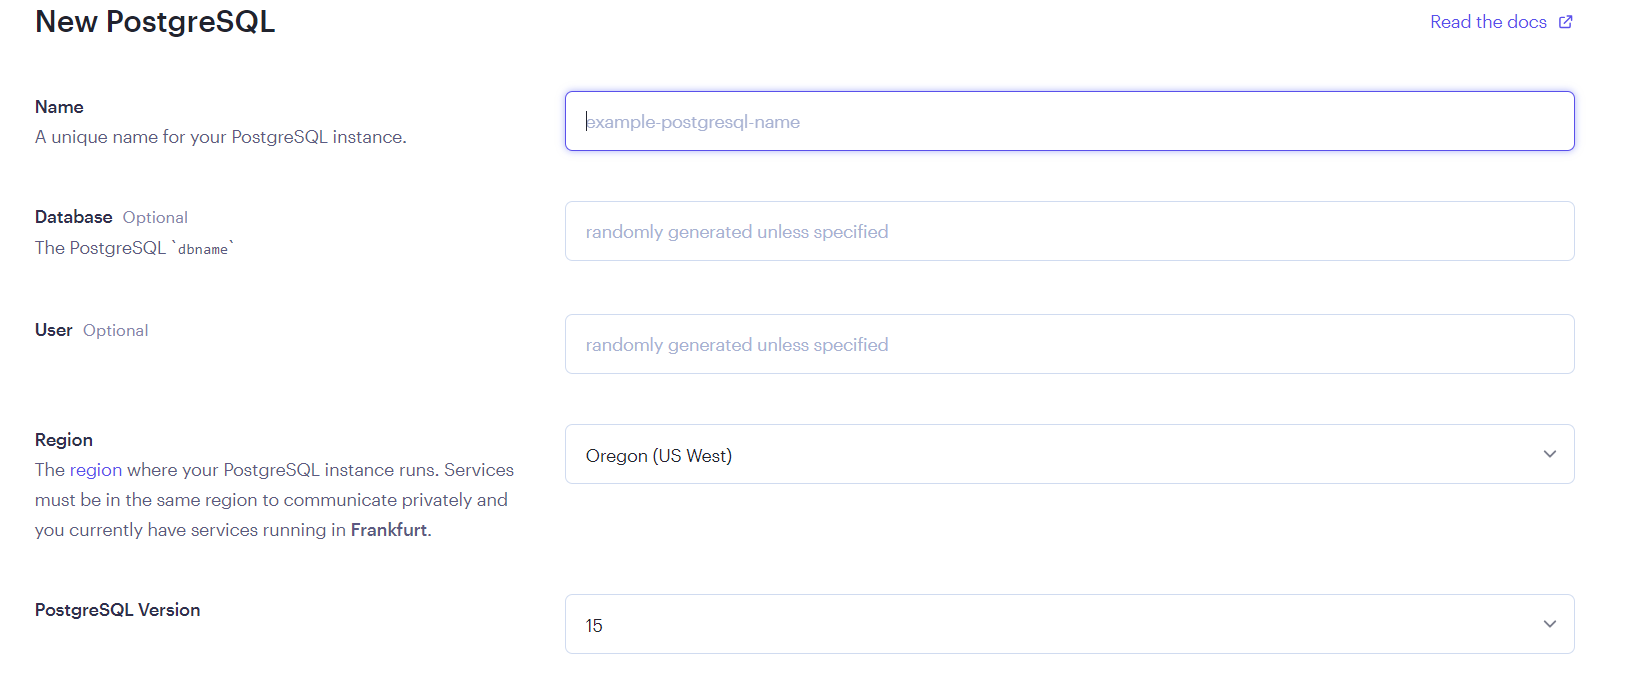
\includegraphics[width=\textwidth]{slike/Baza_podataka1.PNG} %veličina u odnosu na širinu linije
			\caption{Postavljanje i konfiguracija PostgreSQL baze podataka unutar platforme}
			\label{fig:bazapodataka1} %label mora biti drugaciji za svaku sliku
		\end{figure}
		
		Nakon toga Render prikazuje informacije o bazi podataka: ime poslužitelja (\textit{Hostname}), vrata (\textit{Port}), ime baze podataka (\textit{Database}), korisničko ime PostgreSQL korisnika (\textit{username}), lozinku korisnika (\textit{password}) i URL za povezivanje na bazu podataka. 
		
		\item Konfiguracija pristupa bazi podataka iz aplikacije pgAdmin \\
		Unutar aplikacije pgAdmin potrebno je u izborniku odabrati Servers -> Register.
		
		\begin{figure}[H]
			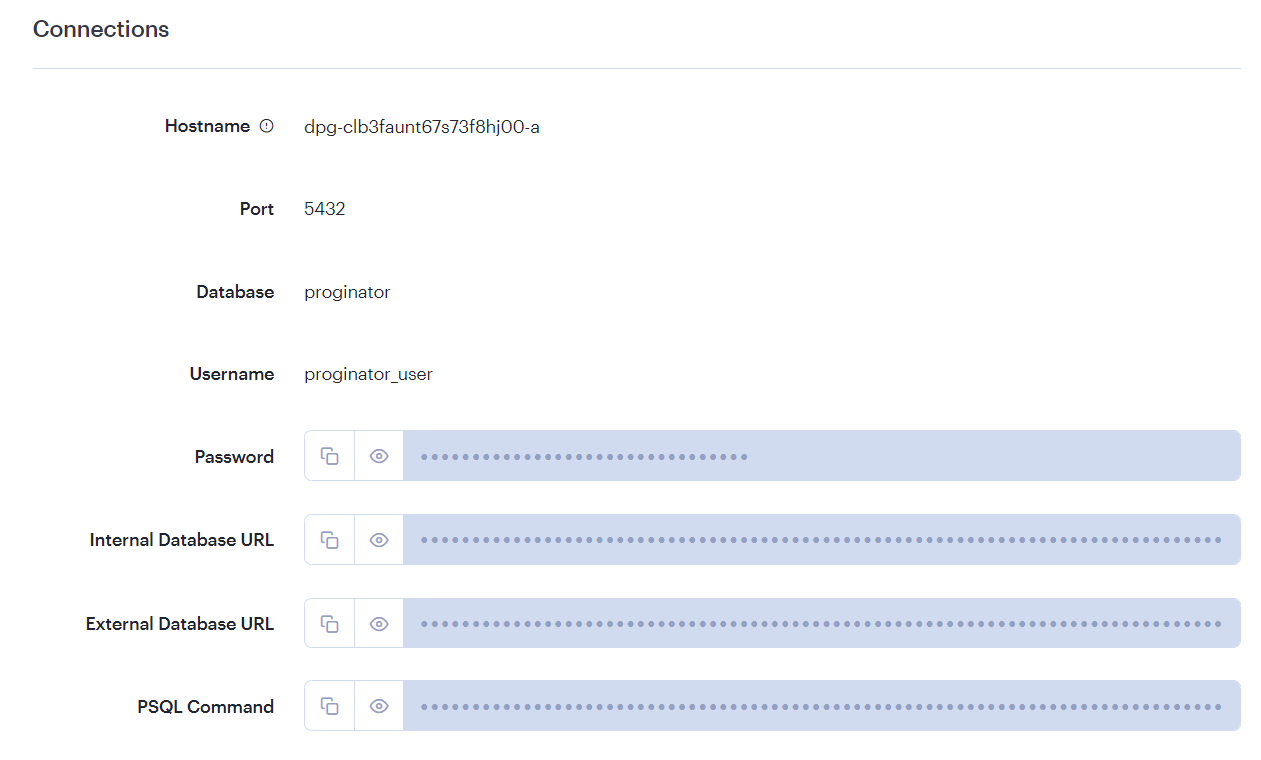
\includegraphics[width=\textwidth]{slike/Baza_podataka2.PNG} %veličina u odnosu na širinu linije
			\caption{Konfiguracija pristupa bazi podataka iz aplikacije pgAdmin}
			\label{fig:bazapodataka2} %label mora biti drugaciji za svaku sliku
		\end{figure}
		
		Nakon toga, potrebno je ispuniti formu s podacima za povezivanje na bazu podataka koje smo dobili u platformi Render.
		\begin{figure}[H]
			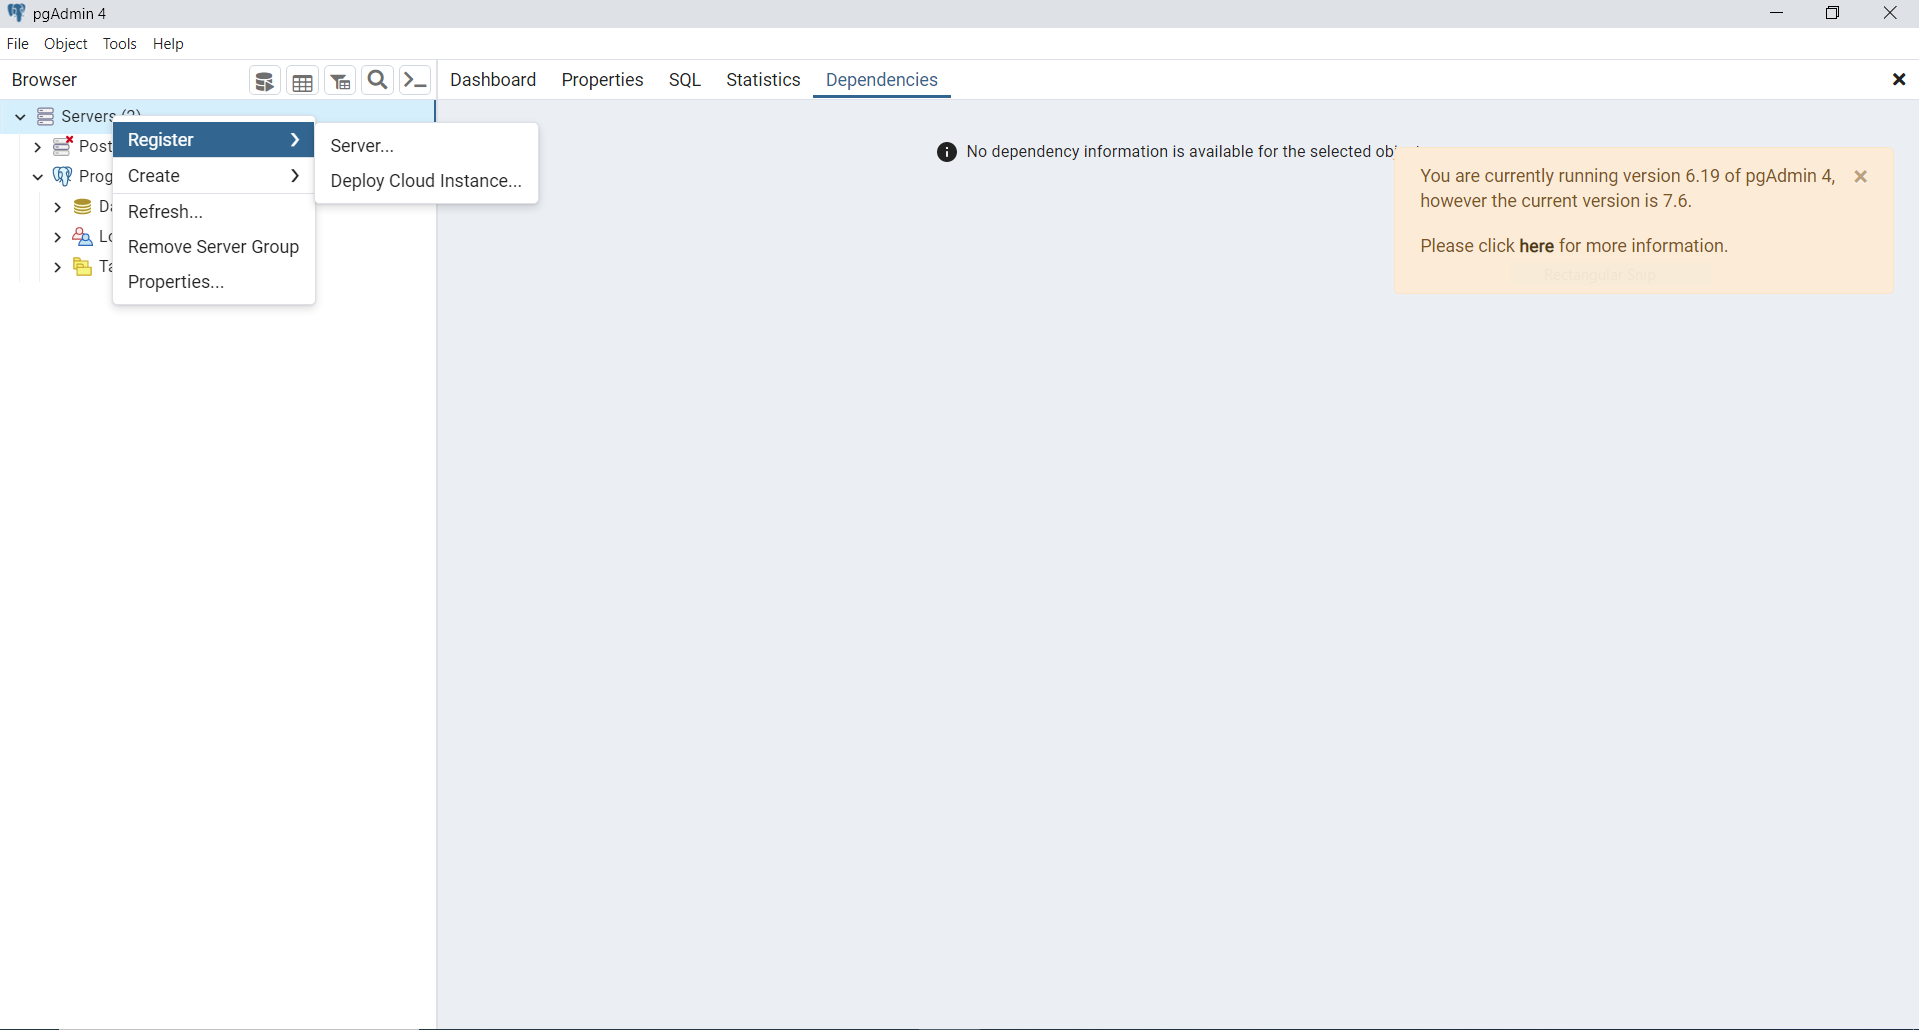
\includegraphics[width=\textwidth]{slike/Baza_podataka3.PNG} %veličina u odnosu na širinu linije
			\caption{Ispunjavanje forme}
			\label{fig:bazapodataka3} %label mora biti drugaciji za svaku sliku
		\end{figure}
		
        \item Incijalizacija baze podataka i stvaranje tablica \\doc
        
        Potrebno je pokrenuti inicijalizacijsku skriptu db\_init.sql koja stvara tablice u bazi podataka.

    				
	 \end{packed_item}


\textbf{Postupak postavljanja backend aplikacije}

\begin{packed_item}
        \item Povezivanje Render web servisa s GitHub repozitorijem \\
        
      \begin{figure}[H]
			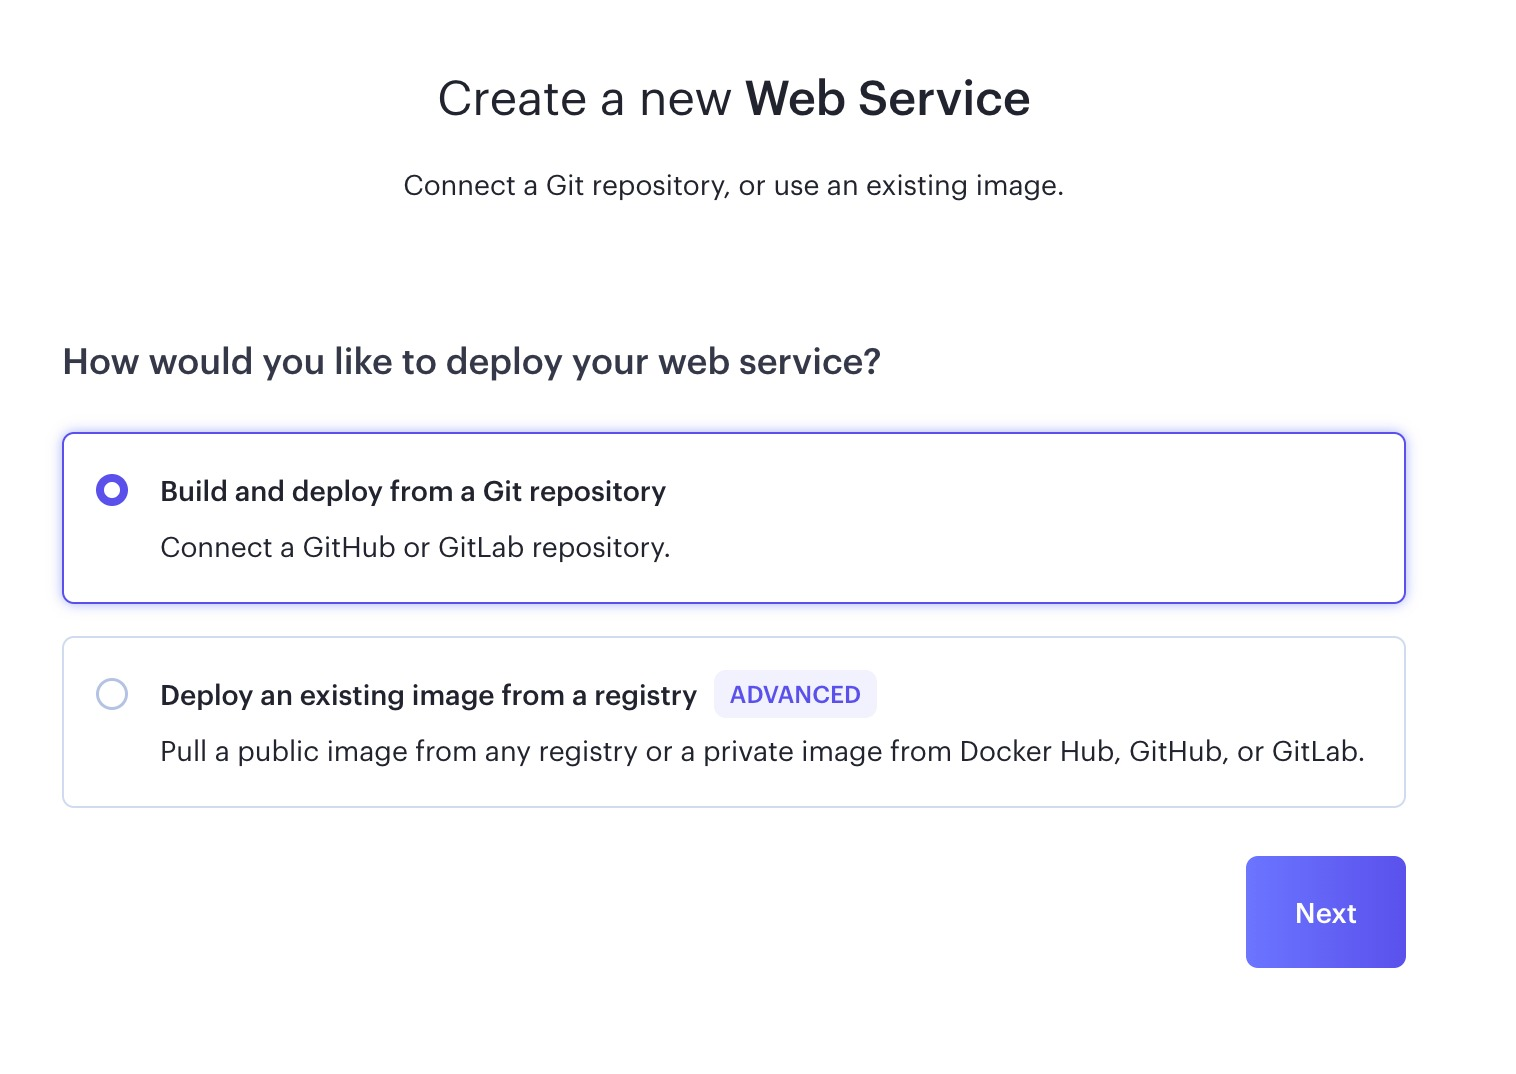
\includegraphics[width=\textwidth]{slike/Backend1.JPG} %veličina u odnosu na širinu linije
			\caption{Povezivanje Render web servisa s GitHub repozitorijem}
			\label{fig:backend1} %label mora biti drugaciji za svaku sliku
		\end{figure}

\begin{figure}[H]
			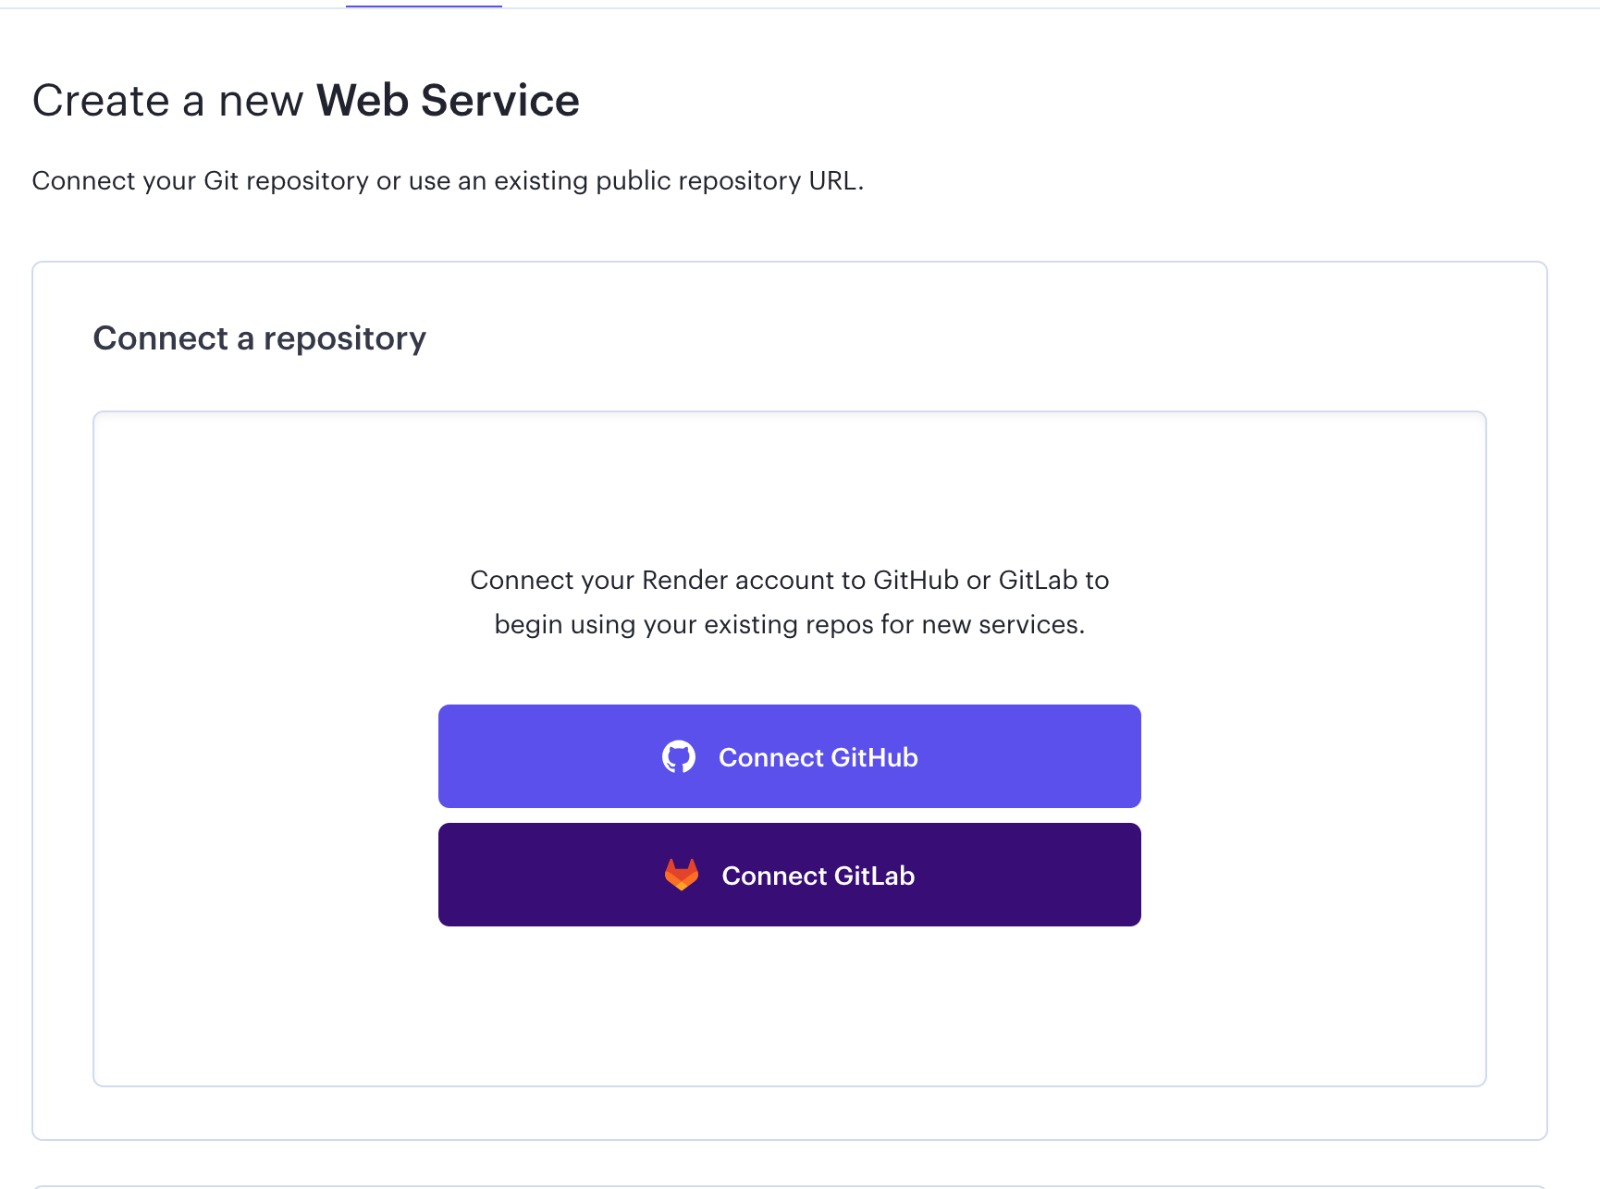
\includegraphics[width=\textwidth]{slike/Backend2.JPG} %veličina u odnosu na širinu linije
			\caption{Povezivanje Render web servisa s GitHub repozitorijem}
			\label{fig:backend2} %label mora biti drugaciji za svaku sliku
		\end{figure}
        
         Render web servis povezujemo s GitHub repozitorijem kako bi Render platforma imala pristup izvornom kodu.
         
        \item Konfiguracija web servisa \\
        
        \begin{figure}
        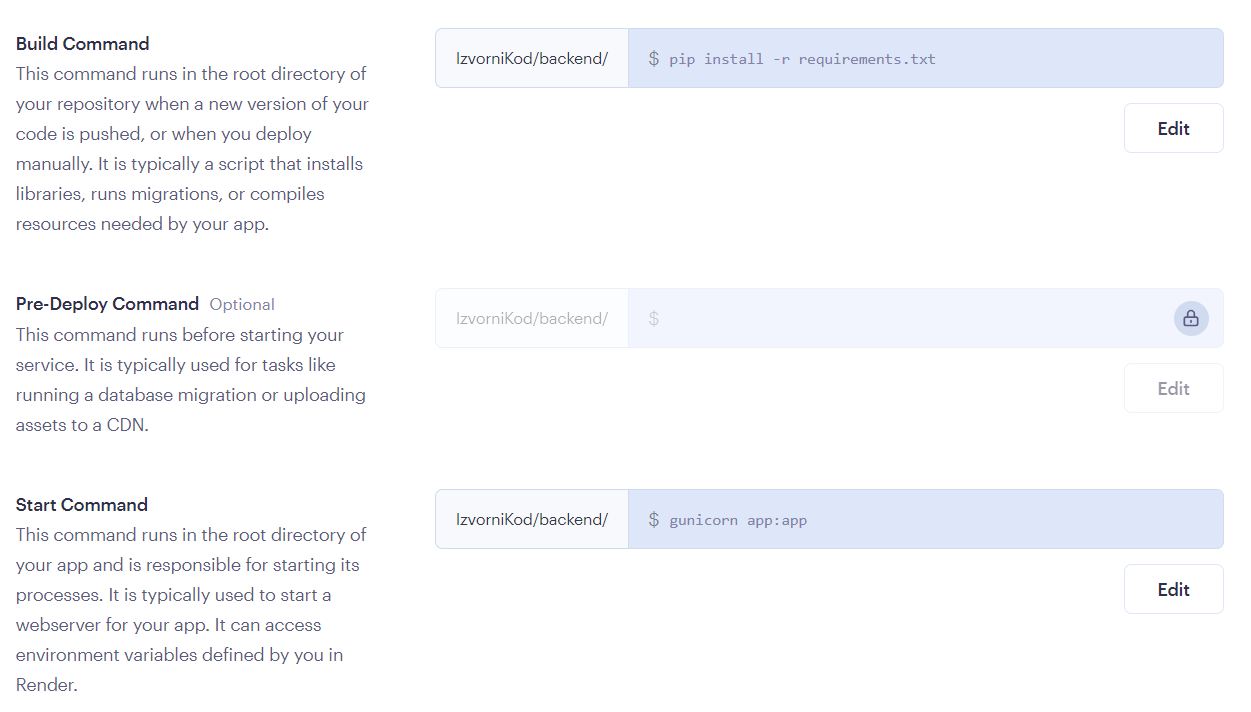
\includegraphics[width=\textwidth]{slike/Backend3.PNG} %veličina u odnosu na širinu linije
			\caption{Konfiguracija web servisa}
			\label{fig:backend3} %label mora biti drugaciji za svaku sliku
		\end{figure}
      
		
        \item Postavljanje varijabli okruženja \\
        \begin{figure}
        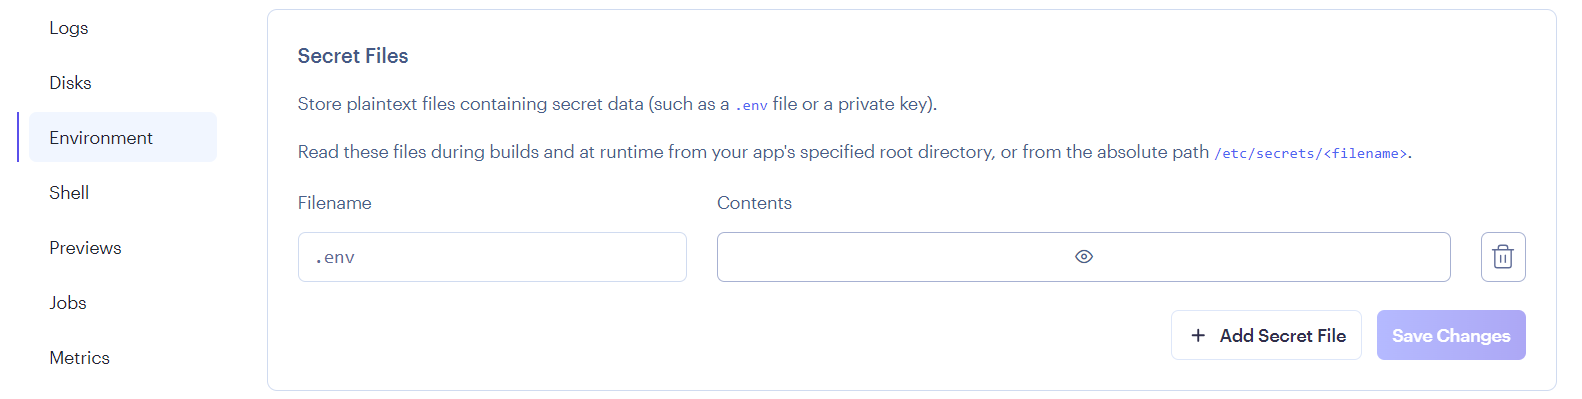
\includegraphics[width=\textwidth]{slike/Backend4.PNG} %veličina u odnosu na širinu linije
			\caption{Postavljanje varijabli okruženja}
			\label{fig:backend4} %label mora biti drugaciji za svaku sliku
		\end{figure}
        
        

\end{packed_item}

\textbf{Postupak postavljanja frontend aplikacije}

\begin{packed_item}
   \item Konfiguracija web servisa \\
   
\begin{figure}[H]
			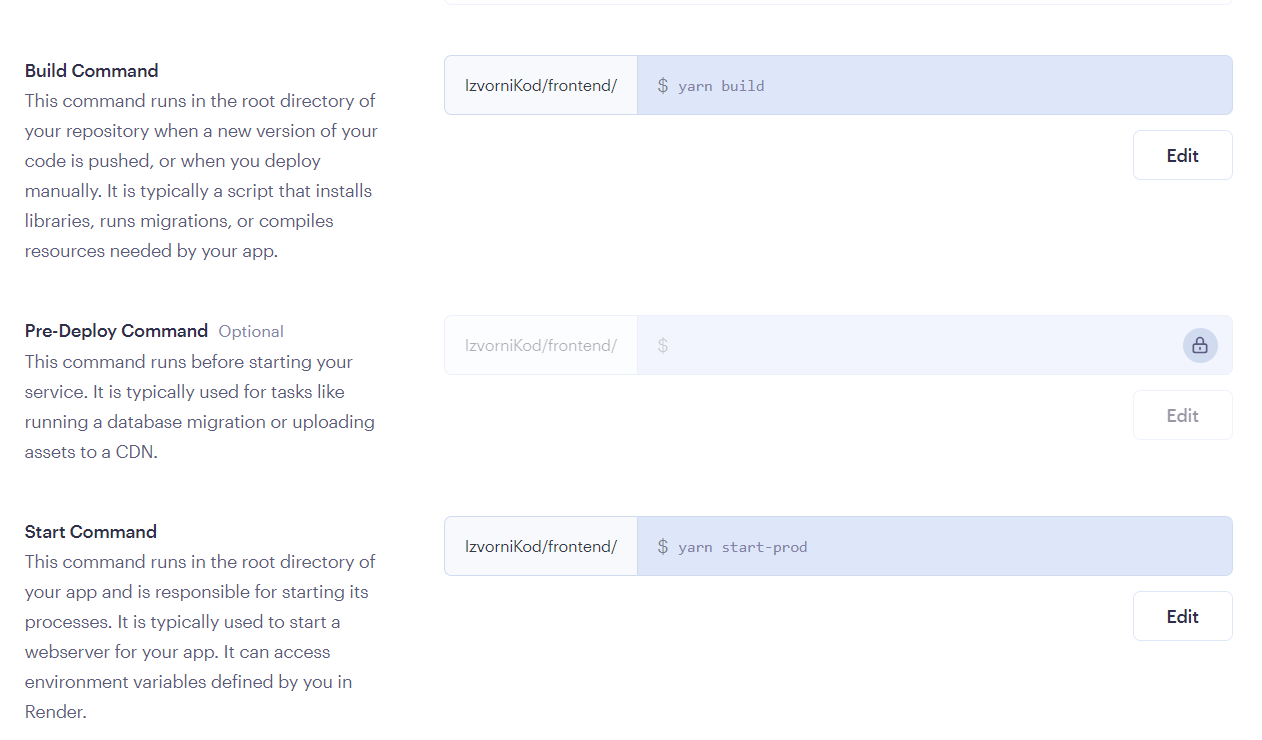
\includegraphics[width=\textwidth]{slike/Frontend1.PNG} %veličina u odnosu na širinu linije
			\caption{Konfiguracija web servisa}
			\label{fig:frontend1} %label mora biti drugaciji za svaku sliku
		\end{figure}
		
   
   Ostali koraci jednaki su koracima postupka postavljanja backend aplikacije.
\end{packed_item}
			
			
			
			\eject 